\chapter{Experiment}
\label{ch:exp}
In the experiment an FTB-300 ``Universal Test System''by EXFO was used to characterize optical links and an optical network. To perform the OTDR measurements an in the FTB-300 integrated FTB-7323B was used. In the first experimets a model standard link is examined. The OTDR is connected to a spool of fiber by a patchcord. Another patchcord connects the end of the fiber to another spool of fiber. The end of the fiber is terminated by an open APC connector. 

\section{Effects of OTDR measurement parameters on the measurements}


\section{Effects of a loose connector on the measurements}

\begin{figure}%
\centering
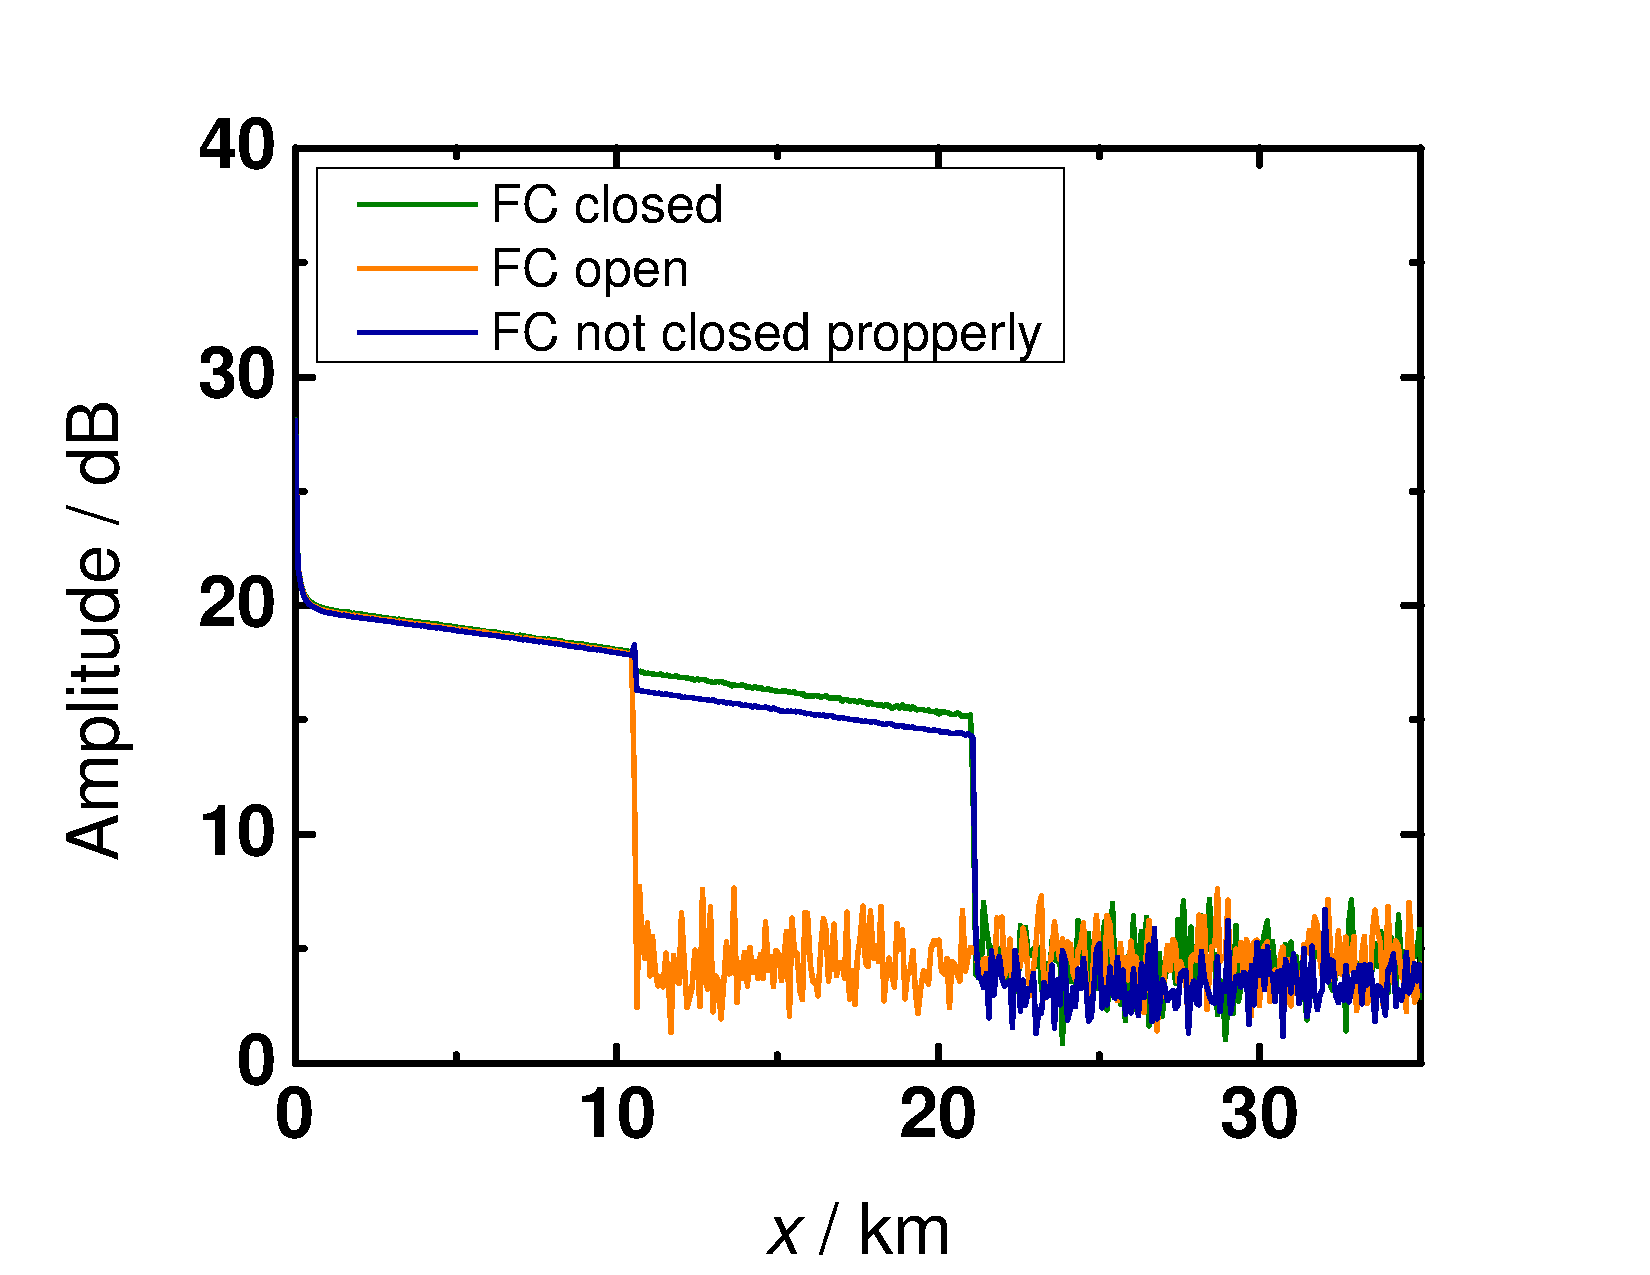
\includegraphics[width=.8\columnwidth]{grafiken/Connector.pdf}%
\caption{}%
\label{fig:connector}%
\end{figure}

In this experiment a connector at the patchcord between the two fibers is loosend. The measurements for this are shown in figure \ref{fig:connector}. The blue curve shows the signal of the link with a closed fiber. When the connector is loosend the losses of the connection increases (green curve). When the connector is loosend further the losses of the connection become so big, that they can't be measured with the OTDR system (orange curve). 

The losses at the connection of a not propperly closed fiber are caused primarily by the end gap between the fibers. Since the light emitted by the end of a fiber spreads conicaly, a higher amount of light misses the core and is not coupled in the other fiber\footnote[4]{http://www.lanshack.com/fiber-optic-tutorial-termination.aspx}.

Using the 4 point measurement of the OTDR the Losses for the closed connector are measured as 0.8~dB. For a not propperly closed connection a loss of 2.6~dB is measured. For a connector loosend further the losses at the connection are greater than 9~dB, so that the backscattering at the end of the fiber couldn't be detected.

\section{Effects of a bend on the measurements}



\section{Effects of an open end with a PC connector}

\section{Analysis of an optical network}



